\section{KYB process} \label{sec:proc:kyb}

\begin{figure}[h!]
  \begin{sequencediagram}
    \newinst{merchant}{\shortstack{Merchant \\
      \\ 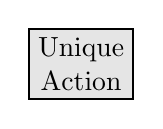
\begin{tikzpicture}
        \node [fill=gray!20,draw=black,thick,align=center] { Unique \\ Action};
      \end{tikzpicture}
    }}
    \newinst[2]{exchange}{\shortstack{Taler (exchange) \\
       \\ \begin{tikzpicture}[shape aspect=.5]
        \tikzset{every node/.style={cylinder,shape border rotate=90, draw,fill=gray!25}}
        \node at (1.5,0) {\shortstack{{{\tiny Database}}}};
       \end{tikzpicture}
    }}
    \newinst[2]{kyb}{\shortstack{KYB provider \\
       \\ \begin{tikzpicture}[shape aspect=.5]
        \tikzset{every node/.style={cylinder,shape border rotate=90, draw,fill=gray!25}}
        \node at (1.5,0) {\shortstack{{{\tiny Database}}}};
       \end{tikzpicture}
    }}

    \postlevel
    \mess[0]{merchant}{{Initial action}}{exchange}
    \begin{callself}{exchange}{Establish KYB requirement}{}
    \end{callself}
    \mess[0]{exchange}{Request new KYB process}{kyb}
    \mess[0]{kyb}{{Process identifier (PI)}}{exchange}
    \mess[0]{exchange}{{KYB required (PI)}}{merchant}
    \mess[0]{merchant}{{KYB start (PI)}}{kyb}
    \mess[0]{kyb}{{Request identity documentation}}{merchant}
    \mess[0]{merchant}{{Upload identity documentation}}{kyb}
    \begin{callself}{kyb}{Validate documentation}{}
    \end{callself}
    \mess[0]{kyb}{{Share documentation (PI)}}{exchange}
    \mess[0]{kyb}{{Confirm completion}}{merchant}
    \mess[0]{merchant}{{Retry action}}{exchange}
\end{sequencediagram}
  \caption{Deposit interactions between customer, Taler exchange (payment
    service provider) and external KYB provider.  The process can be
    triggered by various {\em actions} described in Chapter~\ref{chap:triggers}.}
  \label{fig:proc:kyb}
\end{figure}

At the beginning of the KYB process, the user needs to specify whether they
are an {\bf individual} (not incorporated) or a {\bf business}.\footnote{In
practice, we expect most owners of bank accounts crossing the KYB threshold to
be businesses, but in principle such a bank account could be owned by an
individual operating a business without a separate legal entity.}  This then
determines which types of attributes are collected in the KYB process
(Table~\ref{table:proc:kyb:individual}
vs. Table~\ref{table:proc:kyb:business}).

\begin{table}
  \caption{Information collected for unincorporated individuals}
  \label{table:proc:kyb:individual}
  \begin{center}
    \begin{tabular}{l|c|r}
      {\bf Type}                 & {\bf Required}    & {\bf Example} \\ \hline \hline
      Surname                    & yes        & Mustermann \\
      First name(s)              & yes        & Max \\
      Date of birth              & yes        & 1.1.1980 \\
      Nationality                & yes        & Swiss \\
      Actual address of domicile & yes        & Seestrasse 3, 8008 Zuerich \\
      Phone number               & no         & +41-123456789 \\
      E-mail                     & no         & me@example.com \\
      Identification document    & yes        & JPG image \\
      Taxpayer identification    & yes        & ZPV Nr. 253'123'456 \\
  \end{tabular}
  \end{center}
\end{table}


\begin{table}
  \caption{Information collected for businesses. Information on individals is
    collected for owners with more than 25\% ownership and for those with
    signature authority for the business.}
  \label{table:proc:kyb:business}
  \begin{center}
    \begin{tabular}{l|c|r}
      {\bf Type}                        & {\bf Required} & {\bf Example}        \\ \hline \hline
      Company name                      & yes        & Mega AG \\
      Registered office                 & yes        & Seestrasse 4, 8008 Zuerich \\
      Company identification document   & yes        & PDF file \\
      Power of attorney arrangement     & yes        & PDF file  \\
      Business registration number      & yes        &  \\
      Business registration document    & yes        & PDF file \\
      Registration authority            & yes        &  \\ \hline
      Authorized person name            & yes        & Max Mustermann \\
      Share/authorization certification & yes        & PDF file \\
      Identification document           & yes        & JPG image \\
      Date of birth                     & yes        & 1.1.1980  \\
      Nationality                       & yes        & Swiss     \\
      E-mail                            & yes        & me@example.com \\
      Phone number                      & no         & +41-123456789  \\
  \end{tabular}
  \end{center}
\end{table}
